%%
%% This is file `sample-authordraft.tex',
%% generated with the docstrip utility.
%%
%% The original source files were:
%%
%% samples.dtx  (with options: `authordraft')
%% 
%% IMPORTANT NOTICE:
%% 
%% For the copyright see the source file.
%% 
%% Any modified versions of this file must be renamed
%% with new filenames distinct from sample-authordraft.tex.
%% 
%% For distribution of the original source see the terms
%% for copying and modification in the file samples.dtx.
%% 
%% This generated file may be distributed as long as the
%% original source files, as listed above, are part of the
%% same distribution. (The sources need not necessarily be
%% in the same archive or directory.)
%%
%% The first command in your LaTeX source must be the \documentclass command.
\documentclass[10pt,sigconf, authordraft]{acmart}

%%
%% \BibTeX command to typeset BibTeX logo in the docs
\AtBeginDocument{%
  \providecommand\BibTeX{{%
    \normalfont B\kern-0.5em{\scshape i\kern-0.25em b}\kern-0.8em\TeX}}}

%% Rights management information.  This information is sent to you
%% when you complete the rights form.  These commands have SAMPLE
%% values in them; it is your responsibility as an author to replace
%% the commands and values with those provided to you when you
%% complete the rights form.
\setcopyright{acmcopyright}
\copyrightyear{2019}
\acmYear{2019}
\acmDOI{10.1145/1122445.1122456}

%% These commands are for a PROCEEDINGS abstract or paper.
\acmConference[DEEM '20]{DEEM '20}{June 30, 2020}{Portland, Oregon}


%%
%% Submission ID.
%% Use this when submitting an article to a sponsored event. You'll
%% receive a unique submission ID from the organizers
%% of the event, and this ID should be used as the parameter to this command.
%%\acmSubmissionID{123-A56-BU3}

%%
%% The majority of ACM publications use numbered citations and
%% references.  The command \citestyle{authoryear} switches to the
%% "author year" style.
%%
%% If you are preparing content for an event
%% sponsored by ACM SIGGRAPH, you must use the "author year" style of
%% citations and references.
%% Uncommenting
%% the next command will enable that style.
%%\citestyle{acmauthoryear}

%%
%% end of the preamble, start of the body of the document source.
\begin{document}

%%
%% The "title" command has an optional parameter,
%% allowing the author to define a "short title" to be used in page headers.
\title{Data Version Control: Open source software for versioning and sharing machine learning projects}

%%
%% The "author" command and its associated commands are used to define
%% the authors and their affiliations.
%% Of note is the shared affiliation of the first two authors, and the
%% "authornote" and "authornotemark" commands
%% used to denote shared contribution to the research.
\author{Gabrielle O'Brien, Ph.D.}
\affiliation{%
  \institution{Iterative, Inc.}
}

\author{Dmitry L. Petrov, Ph.D.}
\affiliation{%
  \institution{Iterative, Inc.}
}

\author{Ivan Shcheklein}
\affiliation{%
  \institution{Iterative, Inc.}
}

\author{Ruslan Kupriev}
\affiliation{%
  \institution{Iterative, Inc.}
}



%%
%% By default, the full list of authors will be used in the page
%% headers. Often, this list is too long, and will overlap
%% other information printed in the page headers. This command allows
%% the author to define a more concise list
%% of authors' names for this purpose.
\renewcommand{\shortauthors}{O'Brien et al.}

%%
%% The abstract is a short summary of the work to be presented in the
%% article.
\begin{abstract}
 This will be the abstract. Will summarize DVC and the principals
 explored herein.
\end{abstract}

%%
%% The code below is generated by the tool at http://dl.acm.org/ccs.cfm.
%% Please copy and paste the code instead of the example below.
%%
\begin{CCSXML}
<ccs2012>
<concept>
<concept_id>10011007.10011006.10011072</concept_id>
<concept_desc>Software and its engineering~Software libraries and repositories</concept_desc>
<concept_significance>500</concept_significance>
</concept>
</ccs2012>
\end{CCSXML}

\ccsdesc[500]{Software and its engineering~Software libraries and repositories}
%%
%% Keywords. The author(s) should pick words that accurately describe
%% the work being presented. Separate the keywords with commas.
\keywords{machine learning, data management, infrastructure, version control}


%%
%% This command processes the author and affiliation and title
%% information and builds the first part of the formatted document.
\maketitle

\section{Introduction}
Maintaining the \textit{provenance} of objects--the history of ownership and modification, as well as how the object was derived--is of paramount importance to designing digital systems for scientific reproducibility \cite{Muniswamy-Reddy2006Provenance-awareSystems}. Furthermore, there is growing consensus that auditable and transparent records of scientific projects and their artifacts, such as datasets used to train models \cite{GebruDatasheetsDatasets}, will be required for ethical and fair machine learning practices. 

Yet architecting systems that maintain provenance has proved challenging for projects involving large datasets, a situation that is increasingly common throughout the sciences and applied engineering domains. Efficient systems for tracking evolving datasets and scientific workflows has been a topic of research for many years \cite{Davidson2007ProvenanceSystems.,Azsoyoglu1995TemporalSurvey,Salzberg1999ComparisonData,Bhattacherjee2015PrinciplesTradeoff}. Today, as machine learning proliferates, the matter has increased in both urgency and complexity: in a recent organization-wide survey of data science and machine learning practitioners, \citet{Amershi2019SoftwareStudy} reported that data management was generally ranked as the greatest technical challenge regardless of the practitioner's experience and training. There are likely several reasons for this. 

First, datasets may be larger than ever before (frequently on the terabyte and petabyte scale) and therefore frequently cannot be versioned in the same way as source code \cite{Bhattacherjee2015PrinciplesTradeoff}. Organizations may have thousands, millions, or even billions of datasets internally, which are shared across teams for various purposes \cite{Halevy2016Goods:Datasets}. For each application, datasets may be transformed in new ways, potentially creating a multitude of related by distinct versions of a dataset within an organization.  Compounding this complexity, modern data-driven projects typically involve a long experimentation stage in which users may iterate over many machine learning model architectures and hyperparameters to optimize for a given metric. The resulting models have complex dependencies with both their source code and training dataset (\citet{Amershi2019SoftwareStudy} call this "complex component entanglement"). 

Researchers have identified several priorities for improving data management practices. First, \citet{Schelter2018OnManagement} contend that \textit{data independence}, or abstraction from physical storage \cite{Tsatalos1996TheIndependence}, is a necessary step towards reducing the number of parts in a machine learning pipeline that must be explicitly "glued together". Secondly, the authors also highlight the heterogeneity of code-bases in machine learning: languages and libraries built around relational algebra may be used to query and load datasets, whereas feature transformations are frequently executed via MapReduce-like transforms. Model training may rely on yet other libraries and even hardware, in the case of deep learning. Thus, it is of considerable interest to develop tools for data and experiment management that are language- and library-agnostic. 

Thirdly, it is also desirable that when meta-data about experiments and datasets is tracked, it is not stored in a separate database but maintained with projects artifacts themselves. As \citet{Muniswamy-Reddy2006Provenance-awareSystems} argues, maintaining distinct logs of metadata in a standalone system introduces the need to enforce consistency and maintain another database. A related issue in machine learning experimentation is that practitioners frequently use file-naming conventions or directory structure to track parallel experiments\cite{Gharibi2019AutomatedExperiments}. This creates introduces unnecessary complexity and overhead: version tracking could be automated if abstraction were used instead. 

A fourth priority is that such tools must be designed with minimal overhead to existing practices. Because of the broad variety in backgrounds and skill sets of individuals who work with machine learning pipelines \cite{Amershi2019SoftwareStudy,Halevy2016Goods:Datasets,Schelter2018OnManagement}, it will be imperative to design software that is integrated with existing standards and not overly-specific to a particular discipline (i.e., data science or systems engineering). 


Here, we present our proposal and implementation for a system of tracking the provenance of machine learning projects, including source code, datasets, and trained binary model files, called Data Version Control (DVC). DVC is intended to meet the goals described here: abstraction from physical infrastructure, language agnosticism, [WHAT DO WE CALL THE QUALITY OF NOT NEEDING FILE SUFFIXES?], and integration with existing software engineering practices. Like the approach of \citet{Bhardwaj2015DataHub:Scale} (DATAHUB), a graph-based approach to provenance tracking is central to our design. Unlike DATAHUB, though, we build around an existing graph-based version control system, Git, to extend software engineering principles to data and machine learning experiment management. The main contributions of this work are a transition to \textit{codifying} artifacts like datasets and binary models so that they can be efficiently versioned. We also demonstrate our approach to data independence, which supports a range of physical storage types, and a design philosophy for iterating over machine learning experiments in parallel. 


%% Is architecture the right term? Trying to give an overview of how DVC works.
\section{The DVC data management model}
\subsection{Data addressing and independence}



\begin{figure}[h]
  \centering
  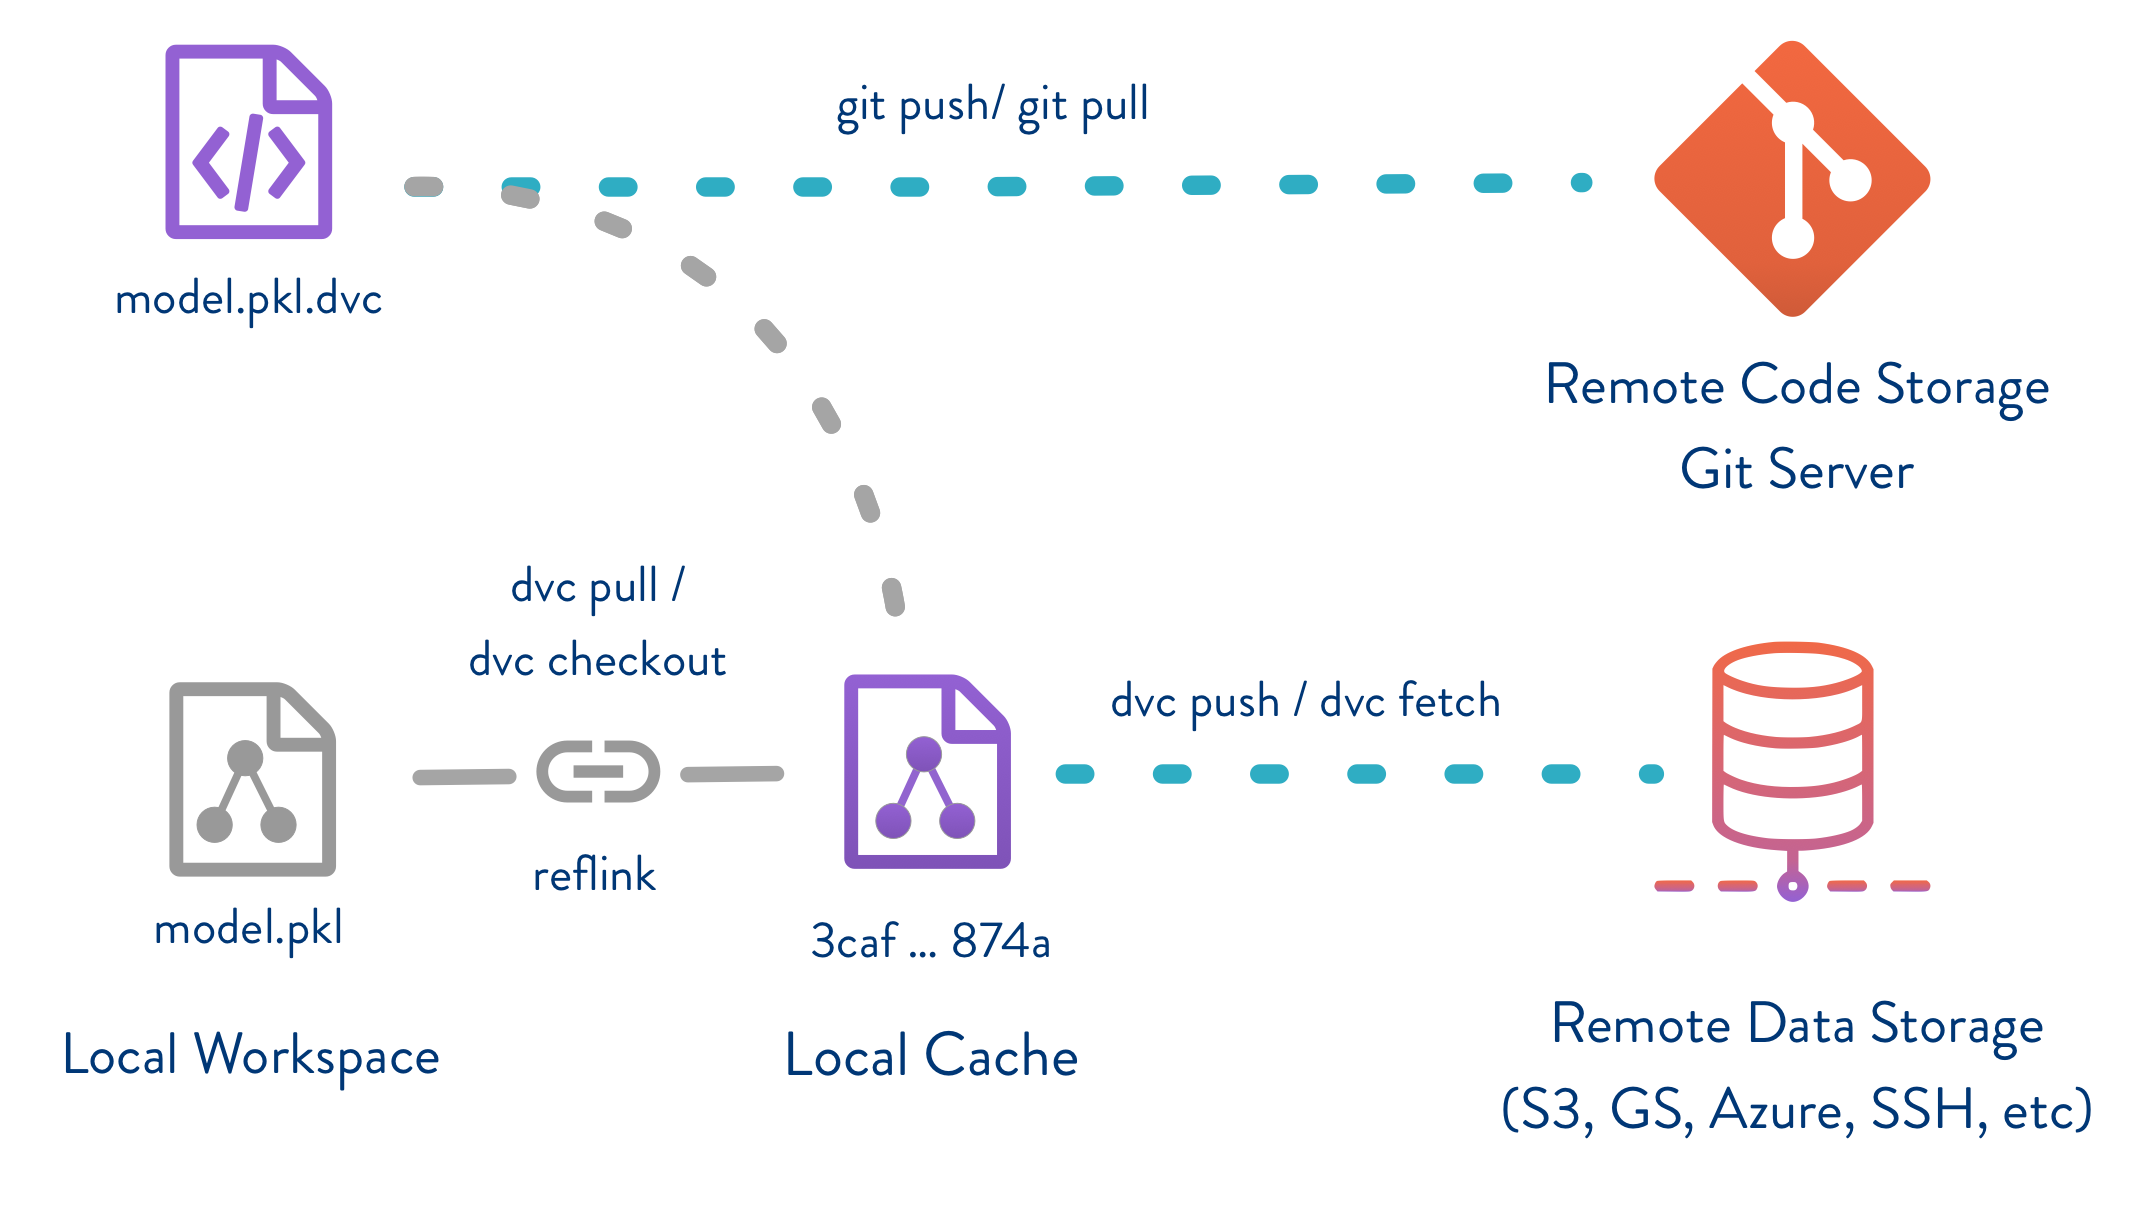
\includegraphics[width=\linewidth]{flow-large.png}
  \caption{A schematic diagram of the DVC workflow}
  \label{fig:fig1}
  \description{Place a description heeeeeeeeeeeeere.}
\end{figure}

DVC is modeled on Git and its distributed architecture, in which source code is pushed and pulled between a \textit{local workspace} and a \textit{remote Git repository}. DVC extends this architecture by adding \textit{remote data storage} (Figure~\ref{fig:fig1}). Importantly, remote data storage is not the repository \textit{to be versioned}; it is a repository for storing versions of large project artifacts from the local workspace (analogous to a remote Git repository). As such, at the start of a project, it will typically be empty. 

DVC is intended to be agnostic to the architecture of remote data storage; it currently supports cloud storage provided by Azure, Amazon Web Services and Google Cloud Storage, as well as SSH, HDFS, HTTP, and network-attached storage.  

\subsubsection{Data independence} Users configure DVC's remote data storage with syntax modeled on Git commands to configure remote code storage. For example:

\begin{verbatim}
    dvc remote add myremote s3://mybucket/myproject
\end{verbatim}


Similar to a Git \verb|config| file, the DVC \verb|config| file stores the physical address of the remote data storage. For the above code example, the DVC \verb|config| file will contain:

\begin{verbatim}
    ['remote "myremote"']
    url = s3://mybucket/myproject
    [core]
    remote = myremote
\end{verbatim}

Consequently, DVC commands can reference the remote data storage by \verb|myremote| instead of its physical address. This abstraction allows the physical address to be changed at any time inside the \verb|config| file without requiring modifications to source code.

\subsubsection{Data as code} 
DVC \textit{codifies} project artifacts such as model files and data, meaning that DVC creates meta-files (\verb|.dvc| files) representing indirect pointers to artifacts in storage. Consider the scenario in Figure~\ref{fig:fig1}, in which a user has trained a model and their local workspace now contains a 3 GB file (\verb|model.pkl|) that cannot be pushed to their GitHub repository due to size restrictions. After bringing this file under DVC's purview (\verb|dvc add model.pkl|), the file \verb|model.pkl.dvc| is created containing the following:

\begin{verbatim}
    md5: 25de4bf3bb47f28f7671627d4fd22a1b
    outs:
    - md5: d41d8cd98f00b204e9800998ecf8427e
      path: model.pkl
      cache: true
      metric: false
      persist: false
\end{verbatim}

This file specifies indirect pointers to the storage location of \verb|model.pkl| that, used in conjunction with the contents of the \verb|config| file, provides a full pointer to the target. The 


The resulting \verb|.dvc| file is versioned by Git exactly as source code. When the user is ready to sync with remote repositories, they will \verb|git commit| and \verb|git push| to remote code storage (such as their GitHub repository). Any \verb|.dvc| files will be synced with remote code storage, but not their corresponding targets (in Figure~\ref{fig:fig1}, \verb|model.pkl.dvc| is synced with remote code storage, but not \verb|model.pkl|.) Lastly, users run \verb|dvc push|, an analogue to \verb|git push|, to copies the contents of \verb|.dvc/cache| to remote data storage (if they are not already present). 

In this way, any artifact of a machine learning project can be versioned with Git while large file contents (and their previous versions) are stored in the remote storage infrastructure of the user's choosing. 

\subsection{Pipelines}


Reproducible pipelines, which include the scripts to preprocess data and carry out classification. Versioning a pipeline may in some cases be more efficient than storing various transformed versions of datasets. 


\section{Research directions}
Currently, DVC provides only raw data management and versioning capabilities: it does not distinguish raw datasets from processed datasets from model binaries, and so does not take advantage of higher levels of abstraction (i.e., dataframes) common in machine learning projects. There is growing interest in new tools to store high-level data objects to data catalogs, feature stores, and model zoos, and future research will investigate how DVC can provide a foundation for these efforts. 

Because DVC is built for efficient transfer of large files between distributed work stations, we expect it will be suitable for various automation scenarios--most commonly, continuous integragtion/continuous deployment (CI/CD). Traditional CI/CD systems are based on code versioning tools, such as Git, and provide the capability to build software artifacts such as executable binary files from source code. In theory, DVC could facilitate dataset transfer in a CI/CD system for automating the training, selection, and deployment of machine learning models. 

Finally, DVC imposes the GitFlow structure on project development: modifications to project components are organized in a graph structure, with Git branches supporting parallel development tracks. This model  software engineering projects where linear structure of code changes does not lead to a complicated graph. A usually project contains only a single branch (usually names master) and a few more temporary feature branches. Branch from feature branches is not a very usual thing in software project. 3rd order branch are really happening. In ML project the structure might be much more complicated due to the trial and error nature of the ML process. A new types of human integration interfaces are needed to simplify the experience.

\section{Conclusions}
We have shown how DVC works.




%%
%% The next two lines define the bibliography style to be used, and
%% the bibliography file.
\bibliographystyle{ACM-Reference-Format}
\bibliography{references}

\end{document}